\section[Introdução]{Introdução}

  O projeto Uma Porto Alegre Alemã tem como objetivo desenvolver um \textit{website} com mapa digital multilíngua (Português, Alemão e opcionalmente Inglês) para divulgar, no Brasil e na Alemanha, as obras do arquiteto alemão Theodor Wiederspahn localizadas em Porto Alegre. A proposta foi pensada para aproximar o público em geral desse patrimônio histórico por meio de uma navegação acessível, organizada e com conteúdo de valor cultural.

  Além do mapa principal, o sistema prevê links para cada edificação com informações mais aprofundadas, como histórico, análise estilística, desenhos técnicos, fotos e modelos tridimensionais. Também está previsto um gerenciamento de conteúdo, permitindo a criação e edição de categorias e materiais multimídia, de forma que a plataforma possa ser atualizada continuamente conforme a evolução do projeto cultural.

  Os \textit{stakeholders} do projeto são Maria Alice Dias, Márcio D'Avila e Raquel Lima, da Escola Politécnica (Curso de Arquitetura e Urbanismo), em uma iniciativa conectada ao contexto de valorização do patrimônio e de aproximação institucional. O projeto está sob orientação do professor José Pedro Schardosin e está sendo desenvolvido no semestre 2026/1, nas sextas-feiras, das 19:15 às 22:30 (6LM6NP), com previsão de entrega para o dia 3 de julho de 2026.

\begin{figure}[H]
    \centering
    \small
    \caption{Time - Uma Porto Alegre Alemã}
    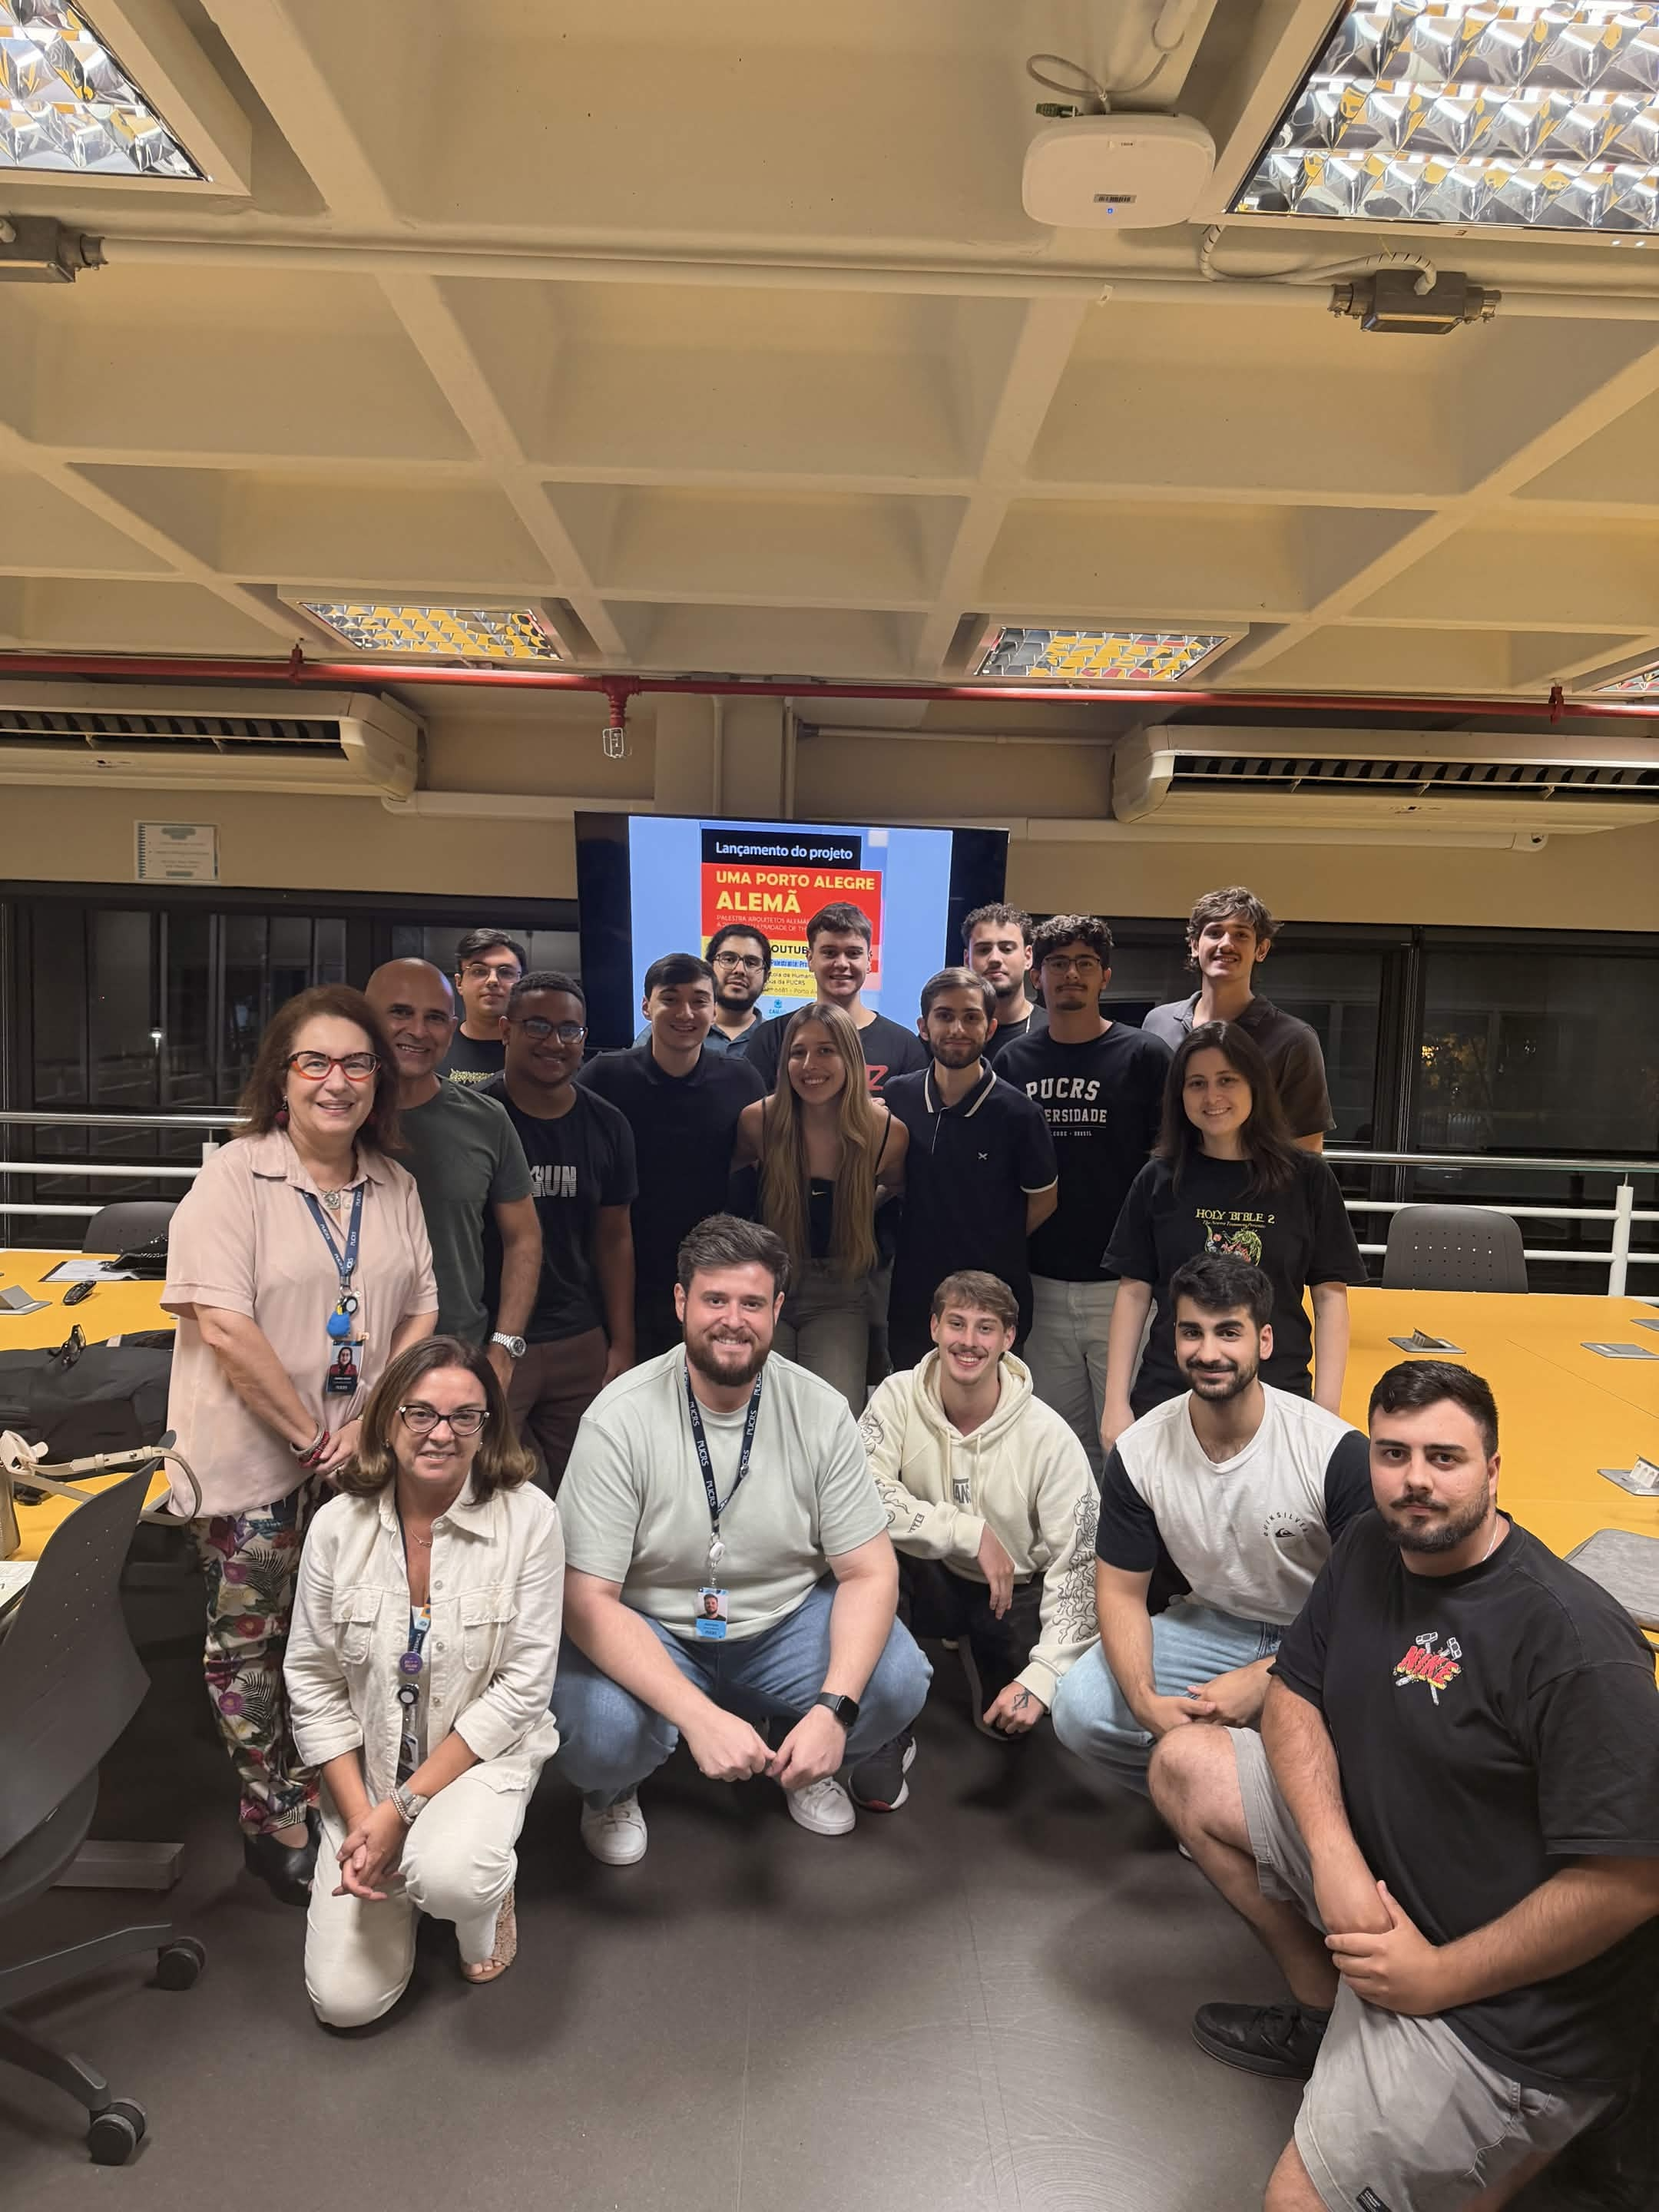
\includegraphics[width=1\linewidth]{conteudo/5 - ages IV/conteudo/figures/EquipeUmaPortoAlegreAlema.jpg}

    Fonte: wiki do projeto
    \label{fig:time-uma-porto-alegre-alema}
\end{figure}
